\chapter{Denlow-X64持续集成测试系统的设计与实现}
\label{cha:intro}

\section{Denlow-X64的背景介绍}

Denlow是以VS2013提供的库为函数库进行编写的一种平台的UEFI BIOS,其编译生成的二进制文件大小为16MB,可以烧录到真实普通PC环境下主板的ROM芯片中以供计算机使用。

在本章中,我们以Denlow平台为例,说明在该种平台下的持续集成测试系统的搭建。最终的完成目标是:在X-64架构(特定的CPU架构)的Denlow平台上,实现对该种架构的UEFI BIOS平台持续集成测试系统的搭建,并且应用到Denlow-X64的实际开发项目中去。

\section{Denlow-X64持续集成测试系统的设计方案}
	\subsection{Denlow-X64持续集成测试系统的环境组成}
		
		Denlow-X64持续集成测试系统的环境组成如图~\ref{fig:Denlow-X64持续集成测试系统的环境组成}所示:
		
		\begin{figure}[H] % use float package if you want it here
			\centering
			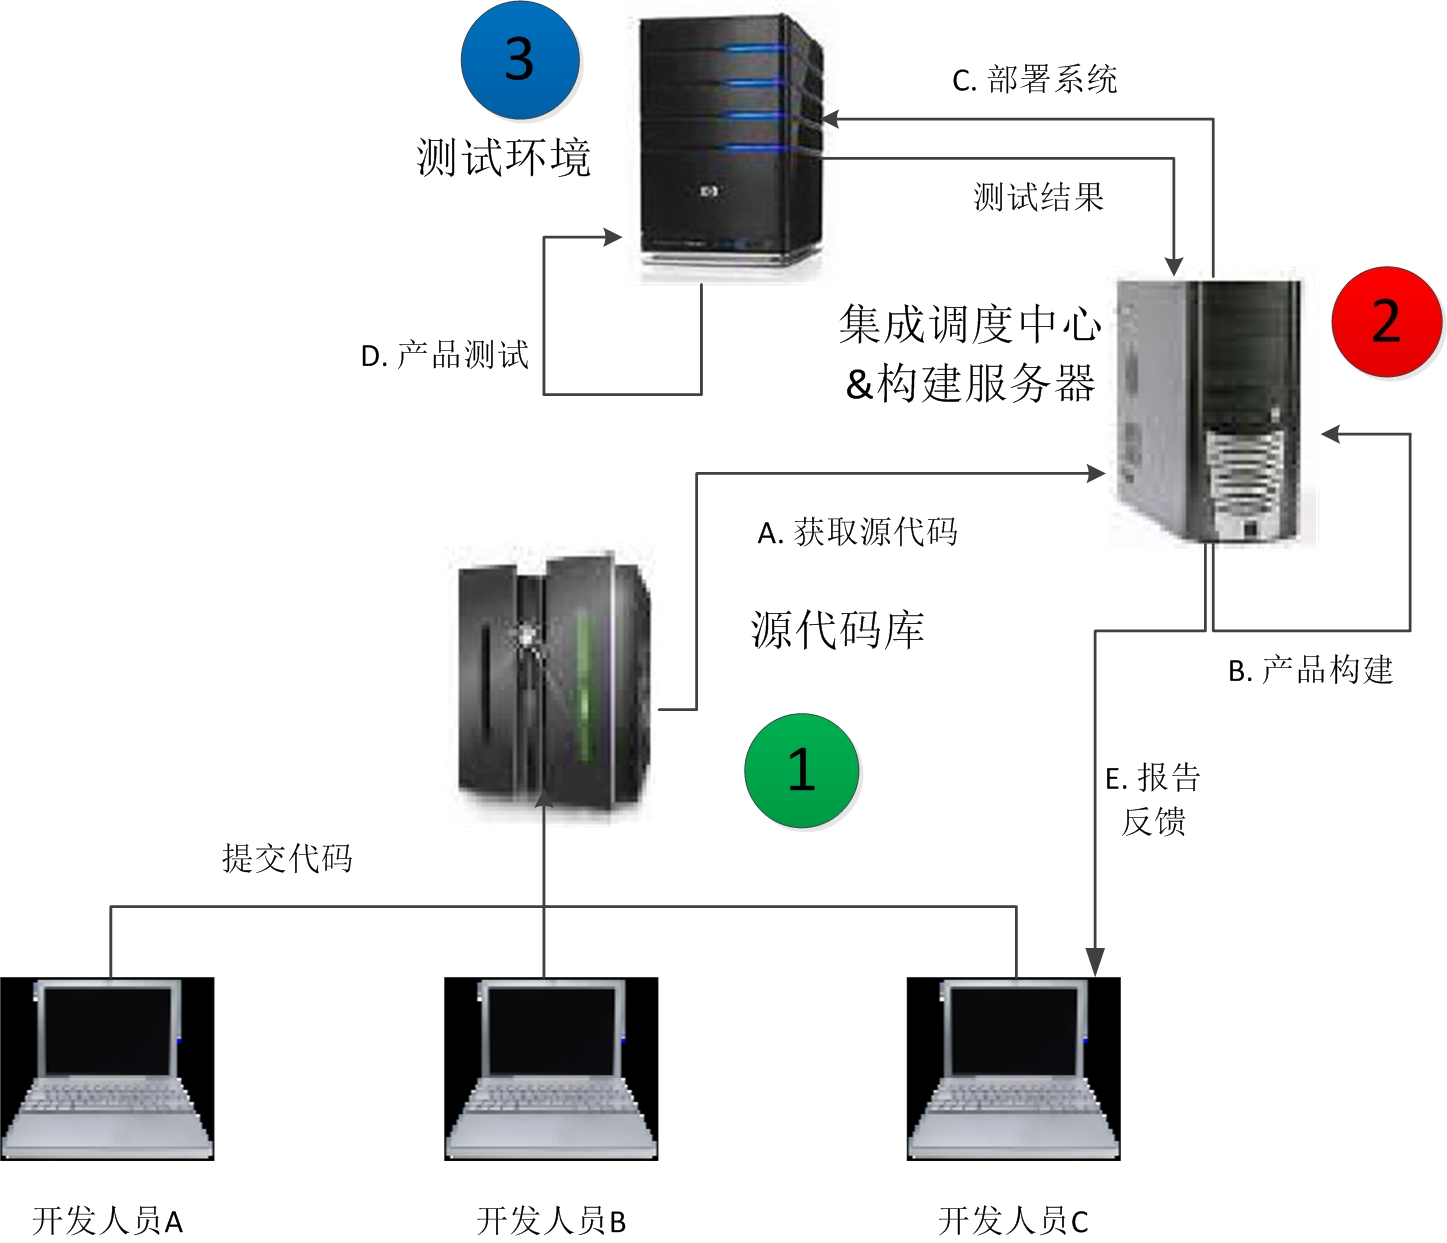
\includegraphics[height=10cm]{chart4/Denlow-X64持续集成测试系统的环境组成}
			\caption{Denlow-X64持续集成测试系统的环境组成}
			\label{fig:Denlow-X64持续集成测试系统的环境组成}
		\end{figure}
		
		其环境主要由源代码库、集成调度中心(同时也是产品构建服务器)和测试环境三部分组成。
		
		\begin{itemize}
			\item 源代码库
			
				源代码库主要负责存储管理Denlow-X64产品的源文件,以便于后续构建服务器对其进行获取和编译构建成所需要的产品进行测试工作。
			\item 集成调度中心(同时也是构建服务器)
				
				集成调度中心主要负责对该持续集成测试系统各功能部分进行调度,例如:
					\begin{itemize}
						\item 通过源代码库下载Denlow-X64的源代码。
						\item 编译构建产品。
						\item 解析测试机端的测试结果。
						\item 报告反馈。
					\end{itemize}
			\item 测试环境
				
				测试环境主要负责测试环境的部署以及对Denlow-X64利用SCT执行功能性测试。
		\end{itemize}
	
	\subsection{Denlow-X64 持续集成测试系统的功能组成}
		
		Denlow-X64持续集成测试系统功能框架组成如图~\ref{fig:Denlow-X64持续集成测试系统的功能框架组成}所示:
		
		\begin{figure}[H] % use float package if you want it here
			\centering
			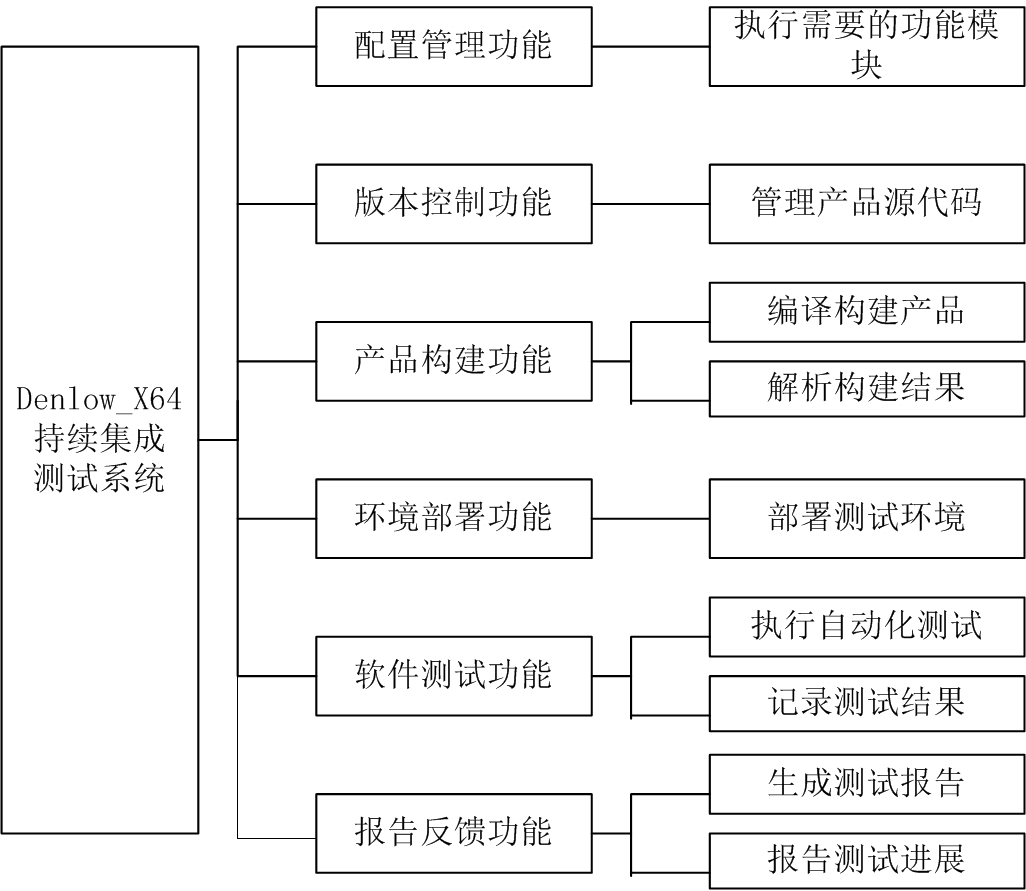
\includegraphics[height=9cm]{chart4/Denlow-X64持续集成测试系统的功能框架组成}
			\caption{Denlow-X64持续集成测试系统的功能框架组成}
			\label{fig:Denlow-X64持续集成测试系统的功能框架组成}
		\end{figure}
		
		其功能框架主要由:1)配置管理功能;2)版本控制功能;3)产品构建功能;4)环境部署功能;5)软件测试功能;6)报告反馈功能六部分模块组成。
	
	\subsection{Denlow-X64 持续集成测试系统的功能流程}
		
		Denlow-X64持续集成测试系统的功能流程如图~\ref{fig:Denlow-X64持续集成测试系统的功能流程}所示:
		
		\begin{figure}[H] % use float package if you want it here
			\centering
			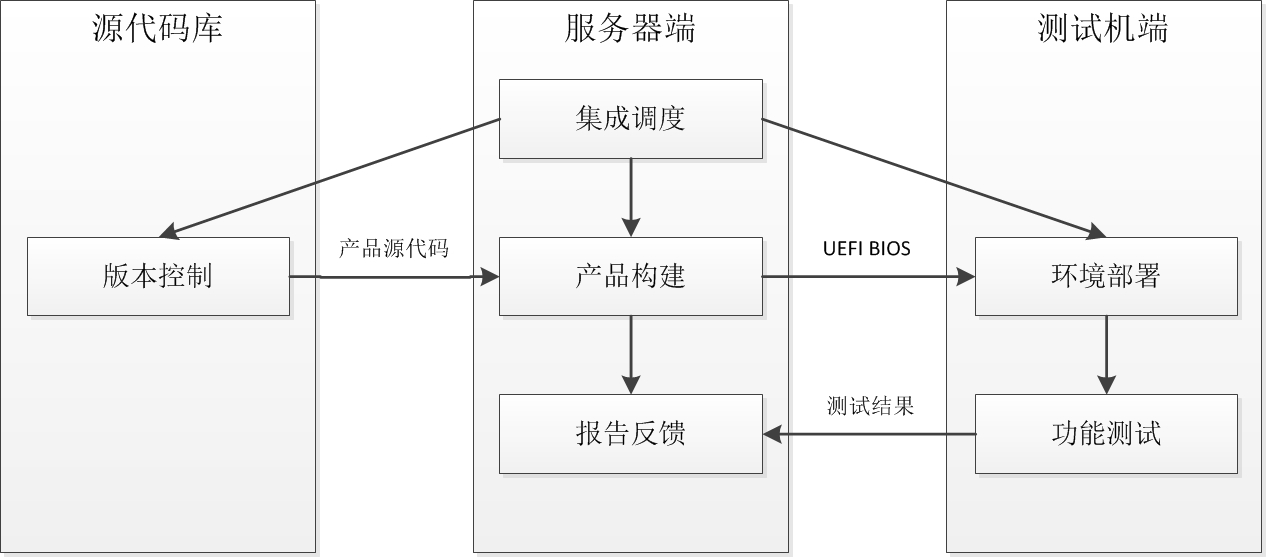
\includegraphics[height=6cm]{chart4/Denlow-X64持续集成测试系统的功能流程}
			\caption{Denlow-X64持续集成测试系统的功能流程}
			\label{fig:Denlow-X64持续集成测试系统的功能流程}
		\end{figure}
		
		服务器负责对整个持续集成测试系统的进行集成调度,其通过版本控制系统从源代码库中获取源文件进行产品构建,将其部署到测试机的环境中,之后利用SCT对产品进行功能性测试,并且将其结果报告、反馈给相关的项目组成员。 

\section{Denlow-X64持续集成测试系统各组成模块的设计与实现}
	
	Denlow-X64持续集成测试系统主要由配置管理、版本控制、产品构建、环境部署、软件测试功能和报告反馈六个模块组成。
	
	由于测试机的操作系统为Windows 2007,服务器的操作系统为Windows Server 2008,测试环境部署以及软件测试需要在测试机UEFI BIOS Shell中进行,因此我们最终选用Windows DOS$\backslash$BAT脚本与UEFI BIOS Shell脚本对该系统进行最终实现。
	
	\subsection{配置管理模块的设计与实现}
		
		为了方便管理Denlow-X64持续集成测试系统各模块是否执行,因此设计和实现本模块用于对系统进行配置和管理。配置文件中的配置信息的设计如图~\ref{fig:配置文件中配置信息的设计}所示:
		
		\begin{figure}[H] % use float package if you want it here
			\centering
			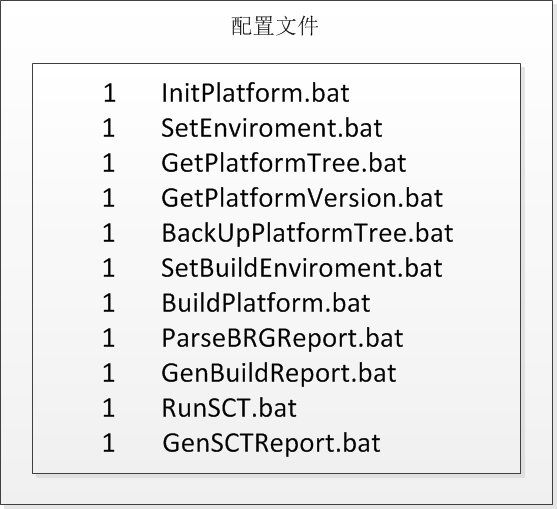
\includegraphics[height=6.5cm]{chart4/配置文件中配置信息的设计}
			\caption{配置文件中配置信息的设计}
			\label{fig:配置文件中配置信息的设计}
		\end{figure}
		
		该配置文件放置在系统主文件夹下的CallingTable.txt文件当中。系统启动之前测试人员对配置文件进行配置,通过修改该配置文件中的内容完成对其的管理:将配置文件中需要执行的模块设置为1,不需要执行的模块设置为0。系统启动时会先解析该配置文件获取相关配置信息,根据其决定所需要执行的模块。如图~\ref{fig:Denlow-X64持续集成测试系统配置管理模块的设计}所示:
		
		\begin{figure}[H] % use float package if you want it here
			\centering
			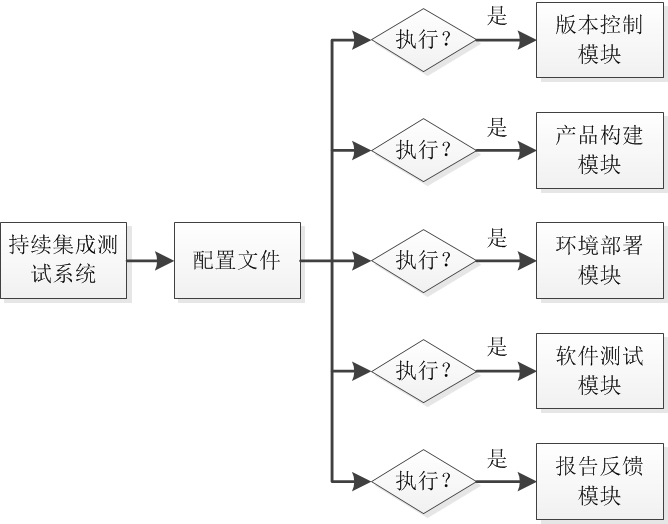
\includegraphics[height=8.5cm]{chart4/Denlow-X64持续集成测试系统配置管理模块的设计}
			\caption{Denlow-X64持续集成测试系统配置管理模块的设计}
			\label{fig:Denlow-X64持续集成测试系统配置管理模块的设计}
		\end{figure}
		
		该模块的主要由main.bat实现,持续集成测试系统启动时首先执行main.bat,进入运行界面,读取配置文件中的配置内容,依次执行配置信息设置为1的各模块脚本,从而实现配置管理模块所需要实现的功能。其中系统的运行界面如图~\ref{fig:Denlow-X64持续集成测试系统集成调度中心的运行界面}所示:
			
		\begin{figure}[H] % use float package if you want it here
			\centering
			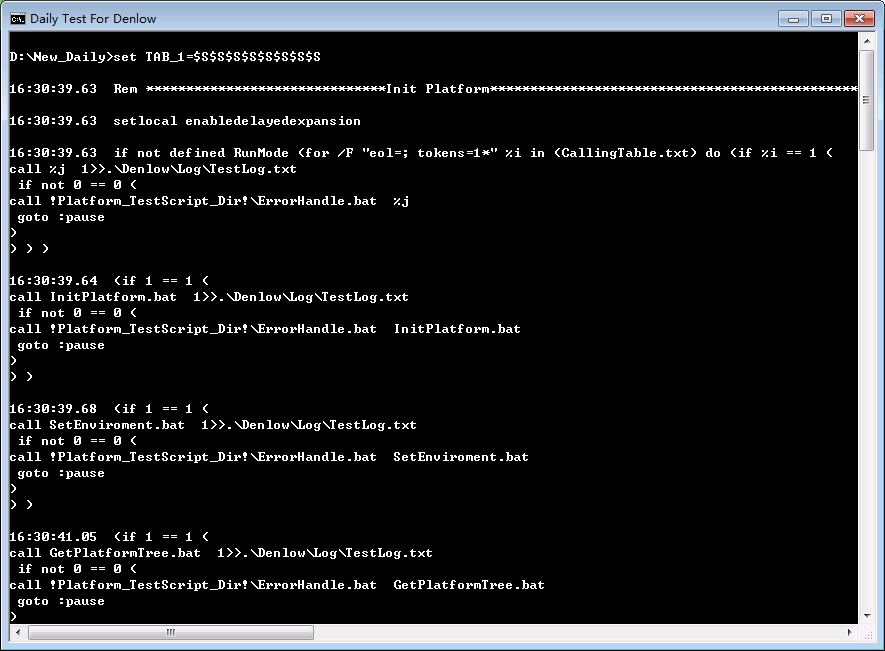
\includegraphics[height=8cm]{chart4/Denlow-X64持续集成测试系统集成调度中心的运行界面}
			\caption{Denlow-X64持续集成测试系统集成调度中心的运行界面}
			\label{fig:Denlow-X64持续集成测试系统集成调度中心的运行界面}
		\end{figure}
	
	\subsection{版本控制模块的设计与实现}
		版本控制模块主要用于管理项目源文件、获取源文件便于后续利用其进行产品构建、获取源文件版本号用于产品构建报告、备份获取到的源文件,其中所用的版本控制系统为Subversion(SVN)。其功能流程如~\ref{fig:Denlow-X64持续集成测试系统版本控制模块的设计}所示:
		
		\begin{figure}[H] % use float package if you want it here
			\centering
			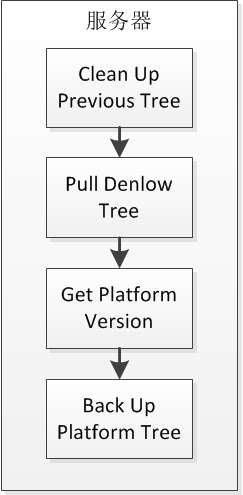
\includegraphics[height=6.5cm]{chart4/Denlow-X64持续集成测试系统版本控制模块的设计}
			\caption{Denlow-X64持续集成测试系统版本控制模块的设计}
			\label{fig:Denlow-X64持续集成测试系统版本控制模块的设计}
		\end{figure}
		
		该模块的主要由三部分脚本共同实现:
		
		\begin{itemize}
			\item GetPlatformTree.bat
			
				GetPlatformTree.bat主要用于:1. Clean Up Previous Tree。2. Pull Denlow Tree。
				\begin{itemize}
					\item Clean Up Previous Tree主要用于清除上一次系统运行时从源代码库中下载的源代码。其先判断源代码文件夹存在与否,若是则删除前一次系统运行时下载的旧版本源文件。
					\item Pull Denlow Tree主要用于利用SVN从源代码库中获取最新版本的源文件。其首先利用SVN从源代码库中尝试获取源文件,若获取成功则结束本脚本执行下一脚本;否则需要利用SVN从源代码库中获取源文件。若该部分执行60次后仍然未能正常获取到产品源文件,则系统获取源文件失败并且结束本部分功能。失败原因可能是由于网络不可用、SVN服务器宕机等非系统因素。
				\end{itemize}
			\item GetPlatformVersion.bat
			
				GetPlatformVersion.bat主要用来获取EDK2和Denlow的版本号等信息,用于后续报告反馈模块。其通过SVN获取EDK2版本号和Denlow的版本号将其赋予相应变量,以便于后续模块对其进行使用。
			\item BackUpPlatformTree.bat
			
				BackUpPlatformTree.bat用于将获取的产品源文件进行备份。
		\end{itemize}
	
	\subsection{产品构建模块的设计与实现}
		
		产品构建模块主要功能是将Denlow-X64的源文件编译构建成为当前版本的UEFI BIOS 产品Denlow.fd,并且生成相应的产品构建报告。其功能流程如图~\ref{fig:Denlow-X64持续集成测试系统产品构建模块的设计}所示:
		
		\begin{figure}[H] % use float package if you want it here
			\centering
			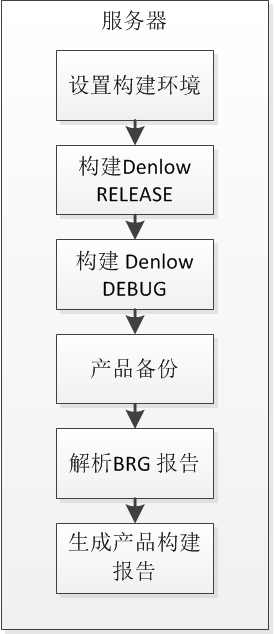
\includegraphics[height=7cm]{chart4/Denlow-X64持续集成测试系统产品构建模块的设计}
			\caption{Denlow-X64持续集成测试系统产品构建模块的设计}
			\label{fig:Denlow-X64持续集成测试系统产品构建模块的设计}
		\end{figure}
		
		该模块的主要由四部分脚本共同实现:
		
		\begin{itemize}
			\item SetBuildEnviroment.bat
				
				SetBuildEnviroment.bat用于设置构建环境以便于后续进行产品构建。SetBuildEnviroment.bat首先调用VS2013安装目录下的vcvarsx86-ia64.bat脚本以设置环境变量,之后调用Denlow源文件中的edksetup.bat脚本以设置产品默认的开发配置。
			\item BuildPlatform.bat
				
				BuildPlatform.bat主要用于编译构建产品,其需要先后构建产品X64的Release版本和Debug版本。其中Release版本的产品需要对其进行环境部署并且进行测试。Build Denlow RELEASE首先清除掉之前一次的产品构建结果与日志,之后进行产品RELEASE版本的构建。若有RELEASE版本的产品出现则判断产品RELEASE版本构建成功,将构建的产品进行备份;否则判断产品构建失败。最后将构建过程中产生的报告文件ReportFile.txt进行备份。
			
				Build Denlow DEBUG用于构建产品的DEBUG版本,判断其是否构建成功,并且对其进行备份。Build Denlow DEBUG首先进行产品DEBUG版本的构建。若有DEBUG版本的产品出现则判断产品DEBUG版本构建成功,将构建的产品进行备份;否则判断产品构建失败。最后将构建过程中产生的报告文件ReportFile.txt进行备份。
			\item ParseBRGReport.bat
				
				产品RELEASE和DEBUG版本的构建过程中会分别产生report-DenlowX64Release.txt与report-DenlowX64Debug.txt。以report-DenlowX64Release.txt为例,其文件头部如图~\ref{fig:report-DenlowX64Release}所示:
				
				\begin{figure}[H] % use float package if you want it here
					\centering
					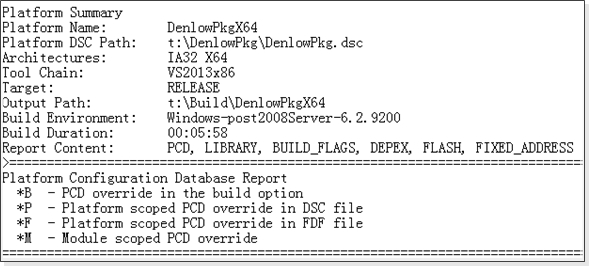
\includegraphics[height=5.5cm]{chart4/report-DenlowX64Release}
					\caption{report-DenlowX64Release}
					\label{fig:report-DenlowX64Release}
				\end{figure}
				
				文件中的Report Content对每一个BRG session进行了总结,ParseBRGReport.bat主要功能是解析该文件,根据Report Content中的session判断每一个BRG session是否正确,并且对判断结果以HTML格式的语句进行记录,如图~\ref{fig:build-results}所示:
				
				\begin{figure}[H] % use float package if you want it here
					\centering
					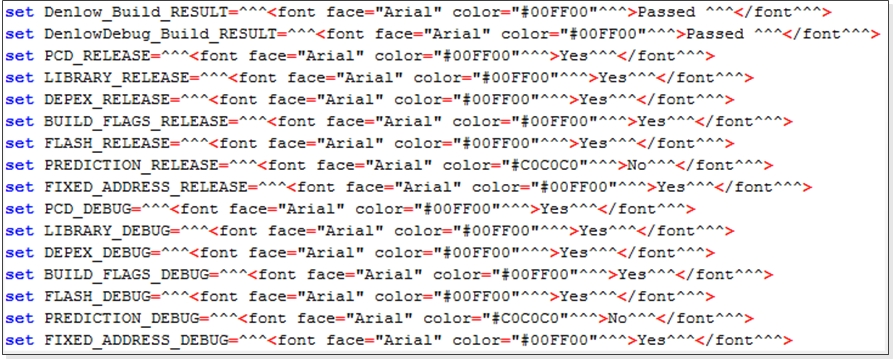
\includegraphics[height=5.5cm]{chart4/build-results}
					\caption{build-results}
					\label{fig:build-results}
				\end{figure}
				
			\item GenBuildReport.bat
				
				GenBuildReport.bat主要依据之前BuildPlatform.bat过程的构建结果判断记录以及ParseBRGReport.bat对BRG session的解析结果,生成网页格式的构建报告以方便QA查看产品构建的结果。其功能流程如图~\ref{fig:GenDenlowBuildReport的功能流程图}所示:
				
				\begin{figure}[H] % use float package if you want it here
					\centering
					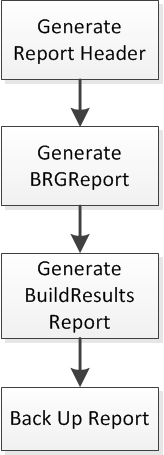
\includegraphics[height=6.5cm]{chart4/GenBuildReport的功能流程图}
					\caption{GenBuildReport的功能流程图}
					\label{fig:GenDenlowBuildReport的功能流程图}
				\end{figure}
				
				GenBuildReport.bat首先生成报告头部,之后依据BRG解析的结果生成报告中BRG报告的相应部分,之后依据之前产品构建结果生成报告中的产品构建的相应部分,最后将整个生成的报告进行备份。
		\end{itemize}
		
	\subsection{环境部署模块的设计与实现}
		
		环境部署模块的主要功能是将之前构建成功的Release版本的UEFI BIOS产品Denlow.fd烧录到测试机主板的ROM芯片中,完成测试环境的部署以便于后续系统对产品的测试。其功能流程如图~\ref{fig:Denlow-X64持续集成测试系统环境部署模块的设计}所示:
		
		\begin{figure}[H] % use float package if you want it here
			\centering
			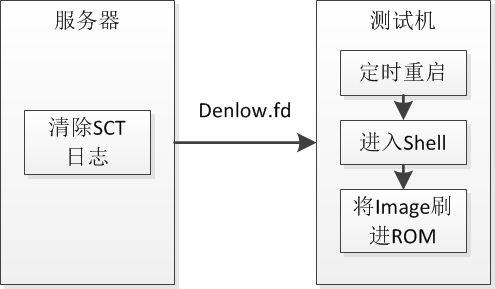
\includegraphics[height=5cm]{chart4/Denlow-X64持续集成测试系统环境部署模块的设计}
			\caption{Denlow-X64持续集成测试系统环境部署模块的设计}
			\label{fig:Denlow-X64持续集成测试系统环境部署模块的设计}
		\end{figure}
		
		该模块功能主要由服务器的脚本RunSCT.bat与测试机端脚本的Startup.nsh共同实现。
		
		\begin{itemize}
			\item Windows映射网络驱动器
				
				为了便于在同一局域网下的服务器和测试机之间传递文件,需要利用Windows映射网络驱动器技术将测试机的共享文件夹映射为服务器的一个映射盘。其设置如图~\ref{fig:利用Windows映射网络驱动器实现文件夹映射}所示:
			
				\begin{figure}[H] % use float package if you want it here
					\centering
					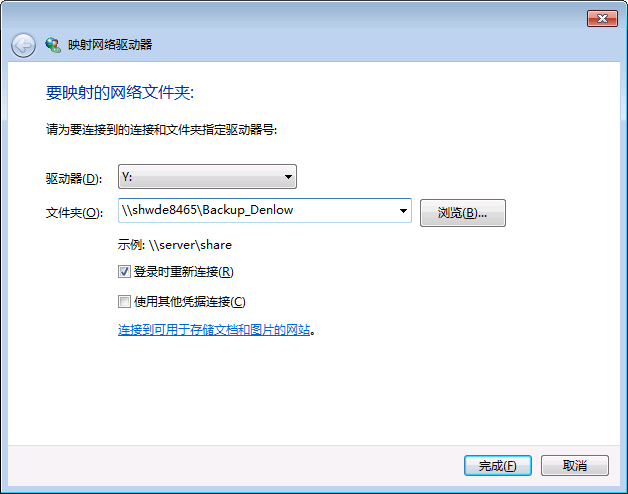
\includegraphics[height=8cm]{chart4/利用Windows映射网络驱动器实现文件夹映射}
					\caption{利用Windows映射网络驱动器实现文件夹映射}
					\label{fig:利用Windows映射网络驱动器实现文件夹映射}
				\end{figure}
			
			\item RunDenlowSCT.bat
				
				RunDenlowSCT.bat用于清除系统上一次执行时的SCT日志,并且将需要测试的产品拷贝到测试机以便于测试机对其进行部署。其功能流程如图~\ref{fig:RunDenlowSCT的功能流程图}所示:
				
				\begin{figure}[H] % use float package if you want it here
					\centering
					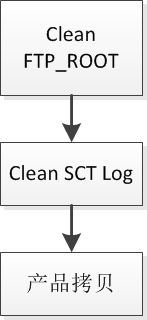
\includegraphics[height=5cm]{chart4/RunDenlowSCT的功能流程图}
					\caption{RunDenlowSCT.bat的功能流程图}
					\label{fig:RunDenlowSCT的功能流程图}
				\end{figure}
				
				Clean FTP-ROOT和Clean SCT Log主要用来清除上一次集成测试时生成的日志文件,以便于后续利用SCT对产品测试时重新生成日志。
				
				Copy Image To Test Computer主要将构建好的Release版本的产品通过设置好的映射盘拷贝到测试机的硬盘中,以便于后续测试环境部署。
			\item 测试机定时重启进入UEFI BIOS Shell环境
				
				该部分主要功能是在服务器产品构建完成并且拷贝到测试机后,测试机定时重启进入UEFI BIOS Shell环境,在Shell环境下利用FirmwareUpdate.efi工具将Image烧录到测试机主板的ROM芯片中,完成测试环境的部署,以便于后续对其进行测试。值得一提的是,UEFI BIOS Shell 有自己的特性,如果计算机开机启动到UEFI BIOS Shell下,在五秒内没有任何操作,则Shell 会自动去检测计算机硬盘中是否有 startup.nsh文件,并且读取该文件中内容执行其中的命令。
				
				为了实现测试机定时重启并且进入UEFI BIOS Shell环境,需要将UEFI BIOS Shell设为开机第一位启动,并且利用Windows 任务计划设置好测试机每天固定的重启时间。定时重启的设置如图~\ref{fig:测试机利用Windows任务计划实现定时重启(一)}、~\ref{fig:测试机利用Windows任务计划实现定时重启(二)}所示:
				
				\begin{figure}[H]
					\begin{minipage}{0.48\textwidth}
					  \centering
					  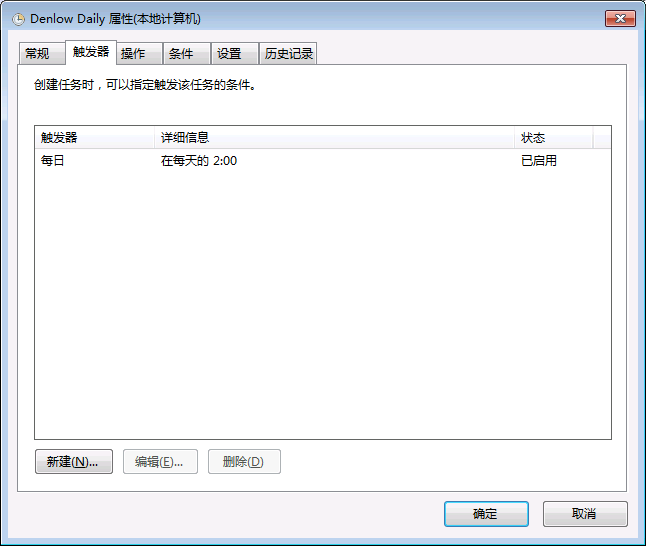
\includegraphics[height=6cm]{chart4/测试机利用Windows任务计划实现定时重启(一)}
					  \caption{测试机利用Windows任务计划实现定时重启(一)}
					  \label{fig:测试机利用Windows任务计划实现定时重启(一)}
					\end{minipage}\hfill
					\begin{minipage}{0.48\textwidth}
					  \centering
					  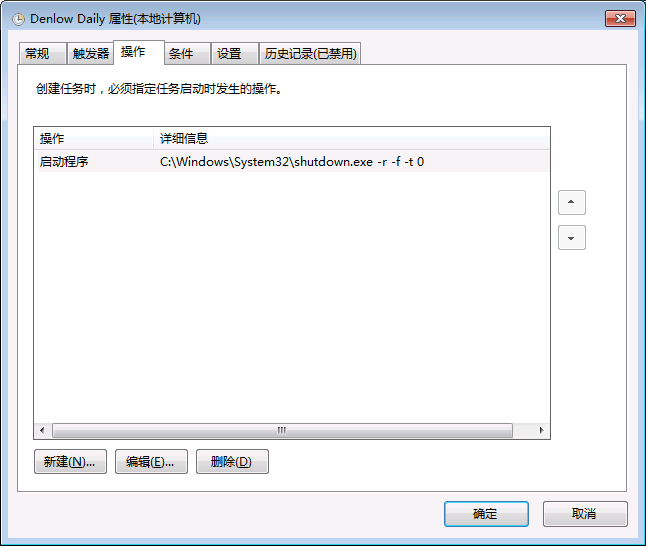
\includegraphics[height=6cm]{chart4/测试机利用Windows任务计划实现定时重启(二)}
					  \caption{测试机利用Windows任务计划实现定时重启(二)}
					  \label{fig:测试机利用Windows任务计划实现定时重启(二)}
					\end{minipage}
				\end{figure}
				
				这样测试机在每天固定时间重启,并且进入UEFI BIOS Shell环境下,读取Startup.nsh中的内容,执行其中的命令从而将Image烧录到测试机主板的ROM芯片中完成测试环境的部署。
			\item Startup.nsh
				
				Startup.nsh主要功能是利用FirmwareUpdate.efi工具将构建好的产品Denlow.fd烧录到测试机主板的ROM芯片中完成测试环境的部署。
				
				测试机首先重置自动化测试工具SCT的环境,之后利用FirmwareUpdate.efi工具将Image文件烧录到测试机主板的ROM芯片中,完成测试环境部署。
		\end{itemize}
					
	\subsection{软件测试模块的设计与实现}
		
		软件测试模块的主要功能是利用自动化测试工具SCT对已经部署好的Denlow UEFI BIOS进行测试,及时发现产品存在的缺陷。其功能流程如图~\ref{fig:Denlow-X64持续集成测试系统软件测试模块的设计}所示:
		
			\begin{figure}[H] % use float package if you want it here
				\centering
				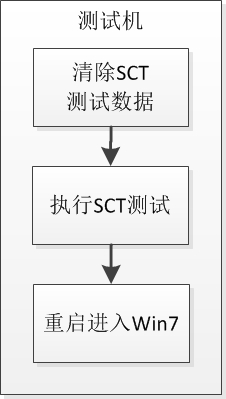
\includegraphics[height=6cm]{chart4/Denlow-X64持续集成测试系统软件测试模块的设计}
				\caption{Denlow-X64持续集成测试系统软件测试模块的设计}
				\label{fig:Denlow-X64持续集成测试系统软件测试模块的设计}
			\end{figure}
		
		自动化测试工具SCT的开发与设计已经在前面章节详细讲述,利用SCT能够实现对产品的自动化测试,并且生成相应的测试日志和初步的测试结果。系统在环境部署模块执行完毕后会重启再次进入UEFI BIOS Shell界面,读取Startup.nsh文件中的内容。因此通过将该部分的操作写入Startup.nsh文件以实现测试的自动化。
	
	\subsection{报告反馈模块的设计与实现}
		
		报告反馈模块的主要功能是在产品构建失败时及时通过邮件向测试人员反馈,以帮助测试人员及时发现问题,并且解析SCT测试的结果,生成相应的报告。其功能流程如图~\ref{fig:报告反馈模块的功能流程图}所示:
		
			\begin{figure}[H] % use float package if you want it here
				\centering
				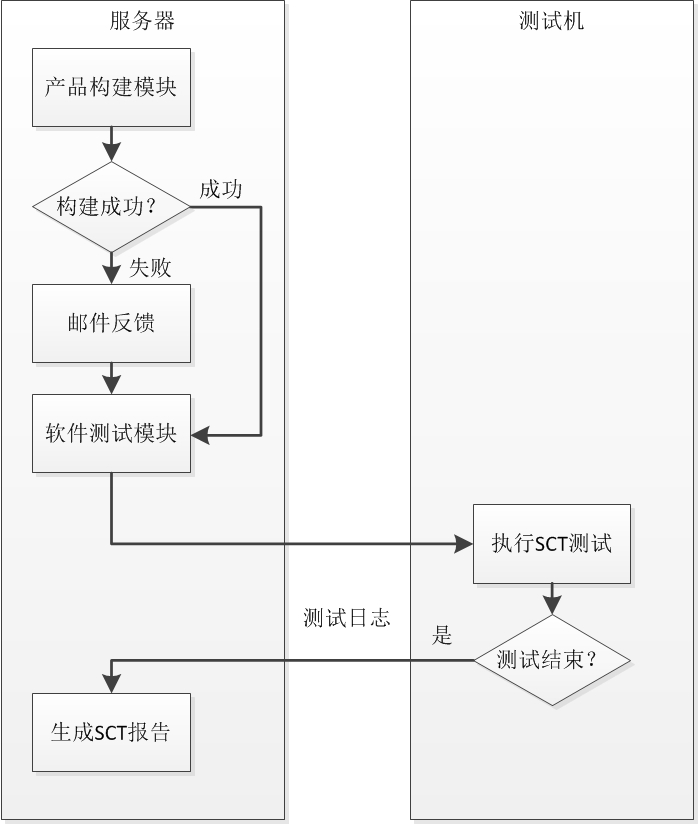
\includegraphics[height=10cm]{chart4/报告反馈模块的功能流程图}
				\caption{报告反馈模块的功能流程图}
				\label{fig:报告反馈模块的功能流程图}
			\end{figure}
		
		该部分的实现主要由MailNotify.bat与GenDenlowSCTReport.bat两部分组成。
		
		\begin{itemize}
			\item MailNotify.bat
				
				MailNotify.bat主要功能是在产品构建失败时及时反馈给测试人员。MailNotify.bat通过SendMail.bat调用已经配置好的SendEmail.exe将产品构建失败的主题和内容通过邮件及时反馈给测试人员,帮助QA快速察觉系统存在的问题,以保障测试活动的顺利开展。
			\item GenDenlowSCTReport.bat
				
				GenDenlowSCTReport.bat负责监测测试机上的SCT测试是否完成,完成后对测试结果进行总结并且生成HTML格式的测试报告,及时报告测试的结果以及产品中存在的缺陷。其功能流程如图~\ref{fig:GenDenlowSCTReport的功能流程图}所示:
				
				\begin{figure}[H] % use float package if you want it here
					\centering
					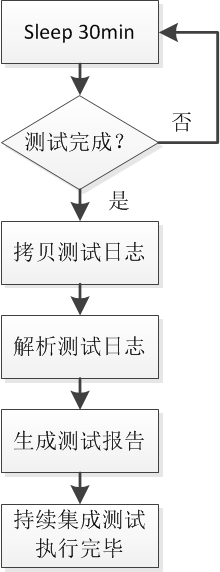
\includegraphics[height=8.5cm]{chart4/GenDenlowSCTReport的功能流程图}
					\caption{GenDenlowSCTReport的功能流程图}
					\label{fig:GenDenlowSCTReport的功能流程图}
				\end{figure}
				
				测试工具SCT完成对UEFI BIOS的测试需要几个小时的时间运行,因此需要以30分钟为单元对测试是否结束进行判断,若测试未完成则休眠30分钟;否则测试结束,利用之前介绍的文件夹映射将测试机上的测试日志拷贝到服务器中,对其进行解析,并且最终生成HTML格式的测试报告,完成系统该轮持续集成所有的任务。
		\end{itemize}
	
	\subsection{系统日志模块的设计与实现}
		
		系统日志模块的主要功能是在系统运行时对其进展进行记录,以帮助系统运行出错时测试人员能够尽快找到原因解决问题。其设计如图~\ref{fig:Denlow-X64持续集成测试系统日志模块的设计}所示:
		
			\begin{figure}[H] % use float package if you want it here
				\centering
				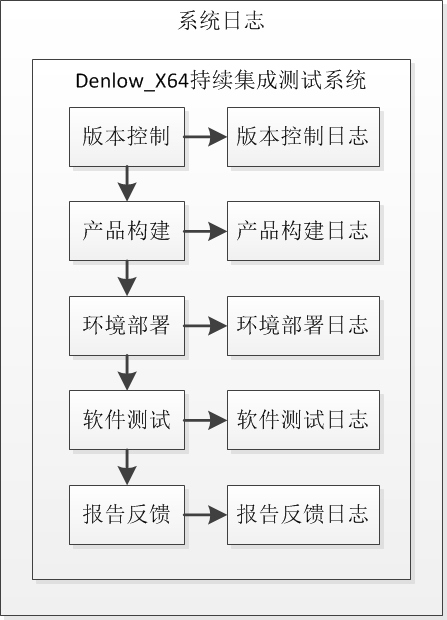
\includegraphics[height=8cm]{chart4/Denlow-X64持续集成测试系统日志模块的设计}
				\caption{Denlow-X64持续集成测试系统日志模块的设计}
				\label{fig:Denlow-X64持续集成测试系统日志模块的设计}
			\end{figure}
		
		系统日志模块产生的日志既包括整个系统运行时的日志,也包括系统每个模块运行时产生的日志。
		
		整个系统运行时的每一个操作和进度都会通过脚本的重定向功能写入到系统日志文件TestLog.txt以供测试人员查看。日志文件格式如图~\ref{fig:系统日志文件TestLog}所示:
		
			\begin{figure}[H] % use float package if you want it here
				\centering
				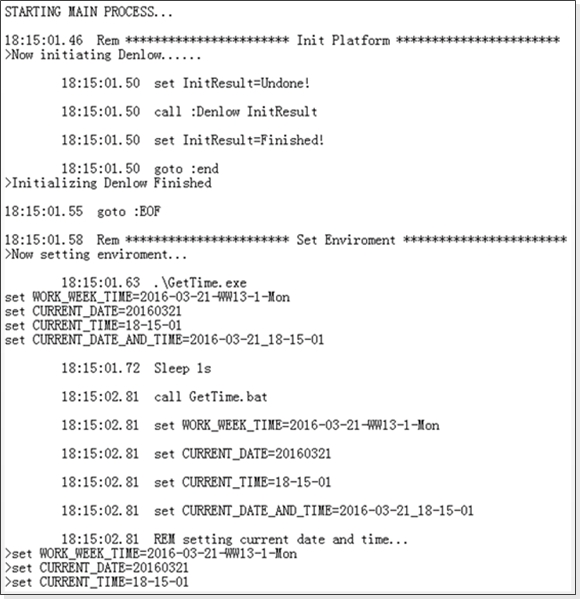
\includegraphics[height=10cm]{chart4/系统日志文件TestLog}
				\caption{系统日志文件TestLog}
				\label{fig:系统日志文件TestLog}
			\end{figure}
		
		系统中每一个模块运行时的操作和进度也会通过重定向写入到各自的日志文件以供测试人员查看。产品构建模块的日志文件BuildLog如图~\ref{fig:产品构建模块日志文件BuildLog}所示:
		
			\begin{figure}[H] % use float package if you want it here
				\centering
				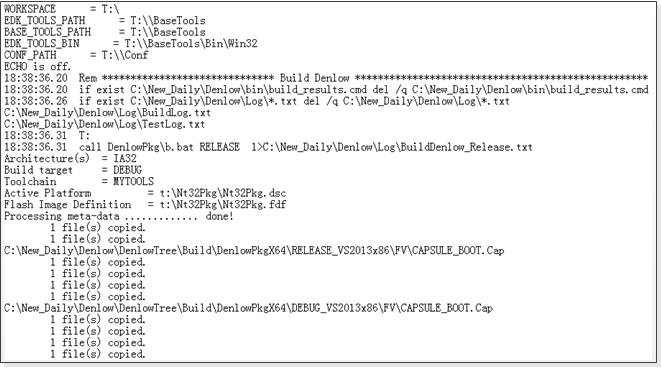
\includegraphics[height=8cm]{chart4/产品构建模块日志文件BuildLog}
				\caption{产品构建模块日志文件BuildLog}
				\label{fig:产品构建模块日志文件BuildLog}
			\end{figure}
		
\section{Denlow-X64持续集成测试系统运行策略的设计与实现}
	\subsection{Denlow-X64持续集成测试系统运行策略的设计}
		
		然而通常Denlow-X64的系统集成完成从源文件的下载、产品的构建到环境的部署,再到软件的测试和报告的反馈这一复杂的过程,需要耗费几个小时的时间,因此时间上并不允许集成的频率过高。为了解决这一矛盾,我们采取的策略便是采用持续集成测试中最低的标准:每日构建。开发人员在白天对产品进行开发和调试,并且将修改的源文件合并提交到源代码库中,而在夜晚,Denlow-X64 持续集成测试系统在无人值守的情况下自动化的运行,对该版本的产品进行构建、部署和测试,并且将测试结果提交报告给相应的人员,这样便能够大大提高整个项目开发的效率。其过程如图~\ref{fig:每日构建(Daily-Build)}所示:
		
		\begin{figure}[H] % use float package if you want it here
			\centering
			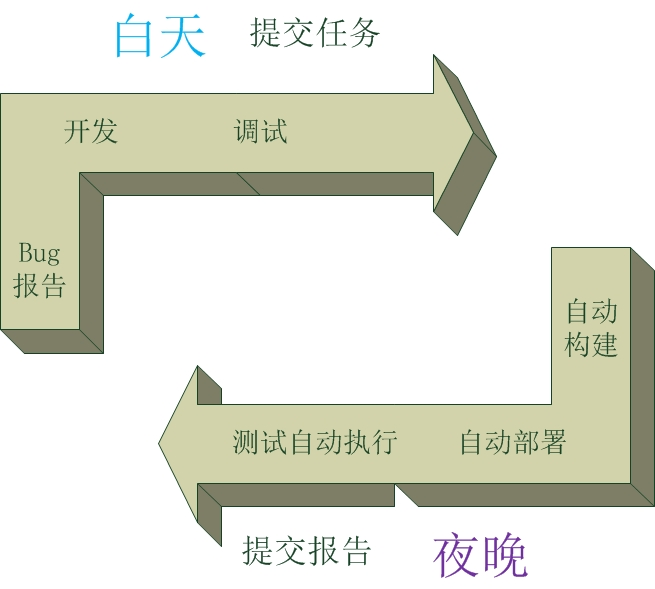
\includegraphics[height=7.5cm]{chart4/每日构建(Daily-Build)}
			\caption{每日构建(Daily Build)}
			\label{fig:每日构建(Daily-Build)}
		\end{figure}
		
	\subsection{Denlow-X64持续集成测试系统运行策略的实现}
		
		为了实现这一需求,利用前文中提到的Windows 任务计划能够有效的做到系统的持续性。系统在当日开发结束提交新版本后,定时启动并且运行,完成持续集成测试的全部任务流程,并且将结果反馈给相关人员。Windows 任务计划对系统的设置如图~\ref{fig:服务器利用Windows任务计划实现持续集成测试系统定时运行(一)}、~\ref{fig:服务器利用Windows任务计划实现持续集成测试系统定时运行(二)}所示:
		
		\begin{figure}[H]
			\begin{minipage}{0.48\textwidth}
			  \centering
			  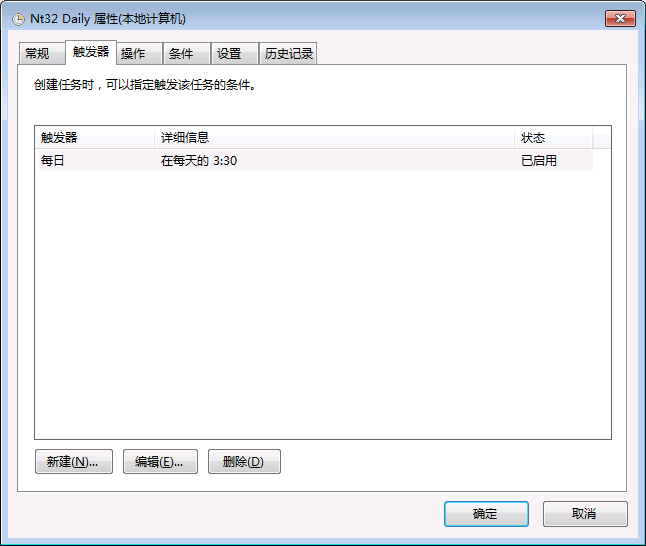
\includegraphics[height=6cm]{chart4/服务器利用Windows任务计划实现持续集成测试系统定时运行(一)}
			  \caption{服务器利用Windows任务计划实现持续集成测试系统定时运行(一)}
			  \label{fig:服务器利用Windows任务计划实现持续集成测试系统定时运行(一)}
			\end{minipage}\hfill
			\begin{minipage}{0.48\textwidth}
			  \centering
			  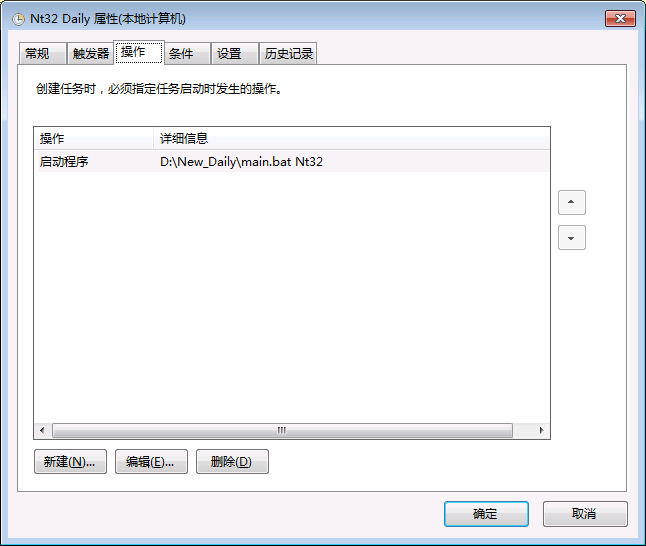
\includegraphics[height=6cm]{chart4/服务器利用Windows任务计划实现持续集成测试系统定时运行(二)}
			  \caption{服务器利用Windows任务计划实现持续集成测试系统定时运行(二)}
			  \label{fig:服务器利用Windows任务计划实现持续集成测试系统定时运行(二)}
			\end{minipage}
		\end{figure}
		
		main.bat是系统的入口点,利用Windows任务计划定时运行main.bat并且传入参数Denlow,即可启动该系统,自动化的完成该轮持续集成测试的任务。
			
\section{Denlow-X64持续集成测试系统的实验结果}
	\subsection{Denlow-X64持续集成测试系统的测试报告}
		
		Denlow-X64持续集成测试系统的报告主要由产品构建报告和产品测试报告两部分组成。
		
		\begin{itemize}
			\item 产品构建报告
				
				产品构建报告负责报告产品构建的情况。以R20406版本的Edk2与R105962版本的Denlow为例,其产品构建报告的结果如图~\ref{fig:R9Prime-Denlow-Build-X64-Report-Edk2-R20406-R9-R105962}所示:
					
				\begin{figure}[H] % use float package if you want it here
					\centering
					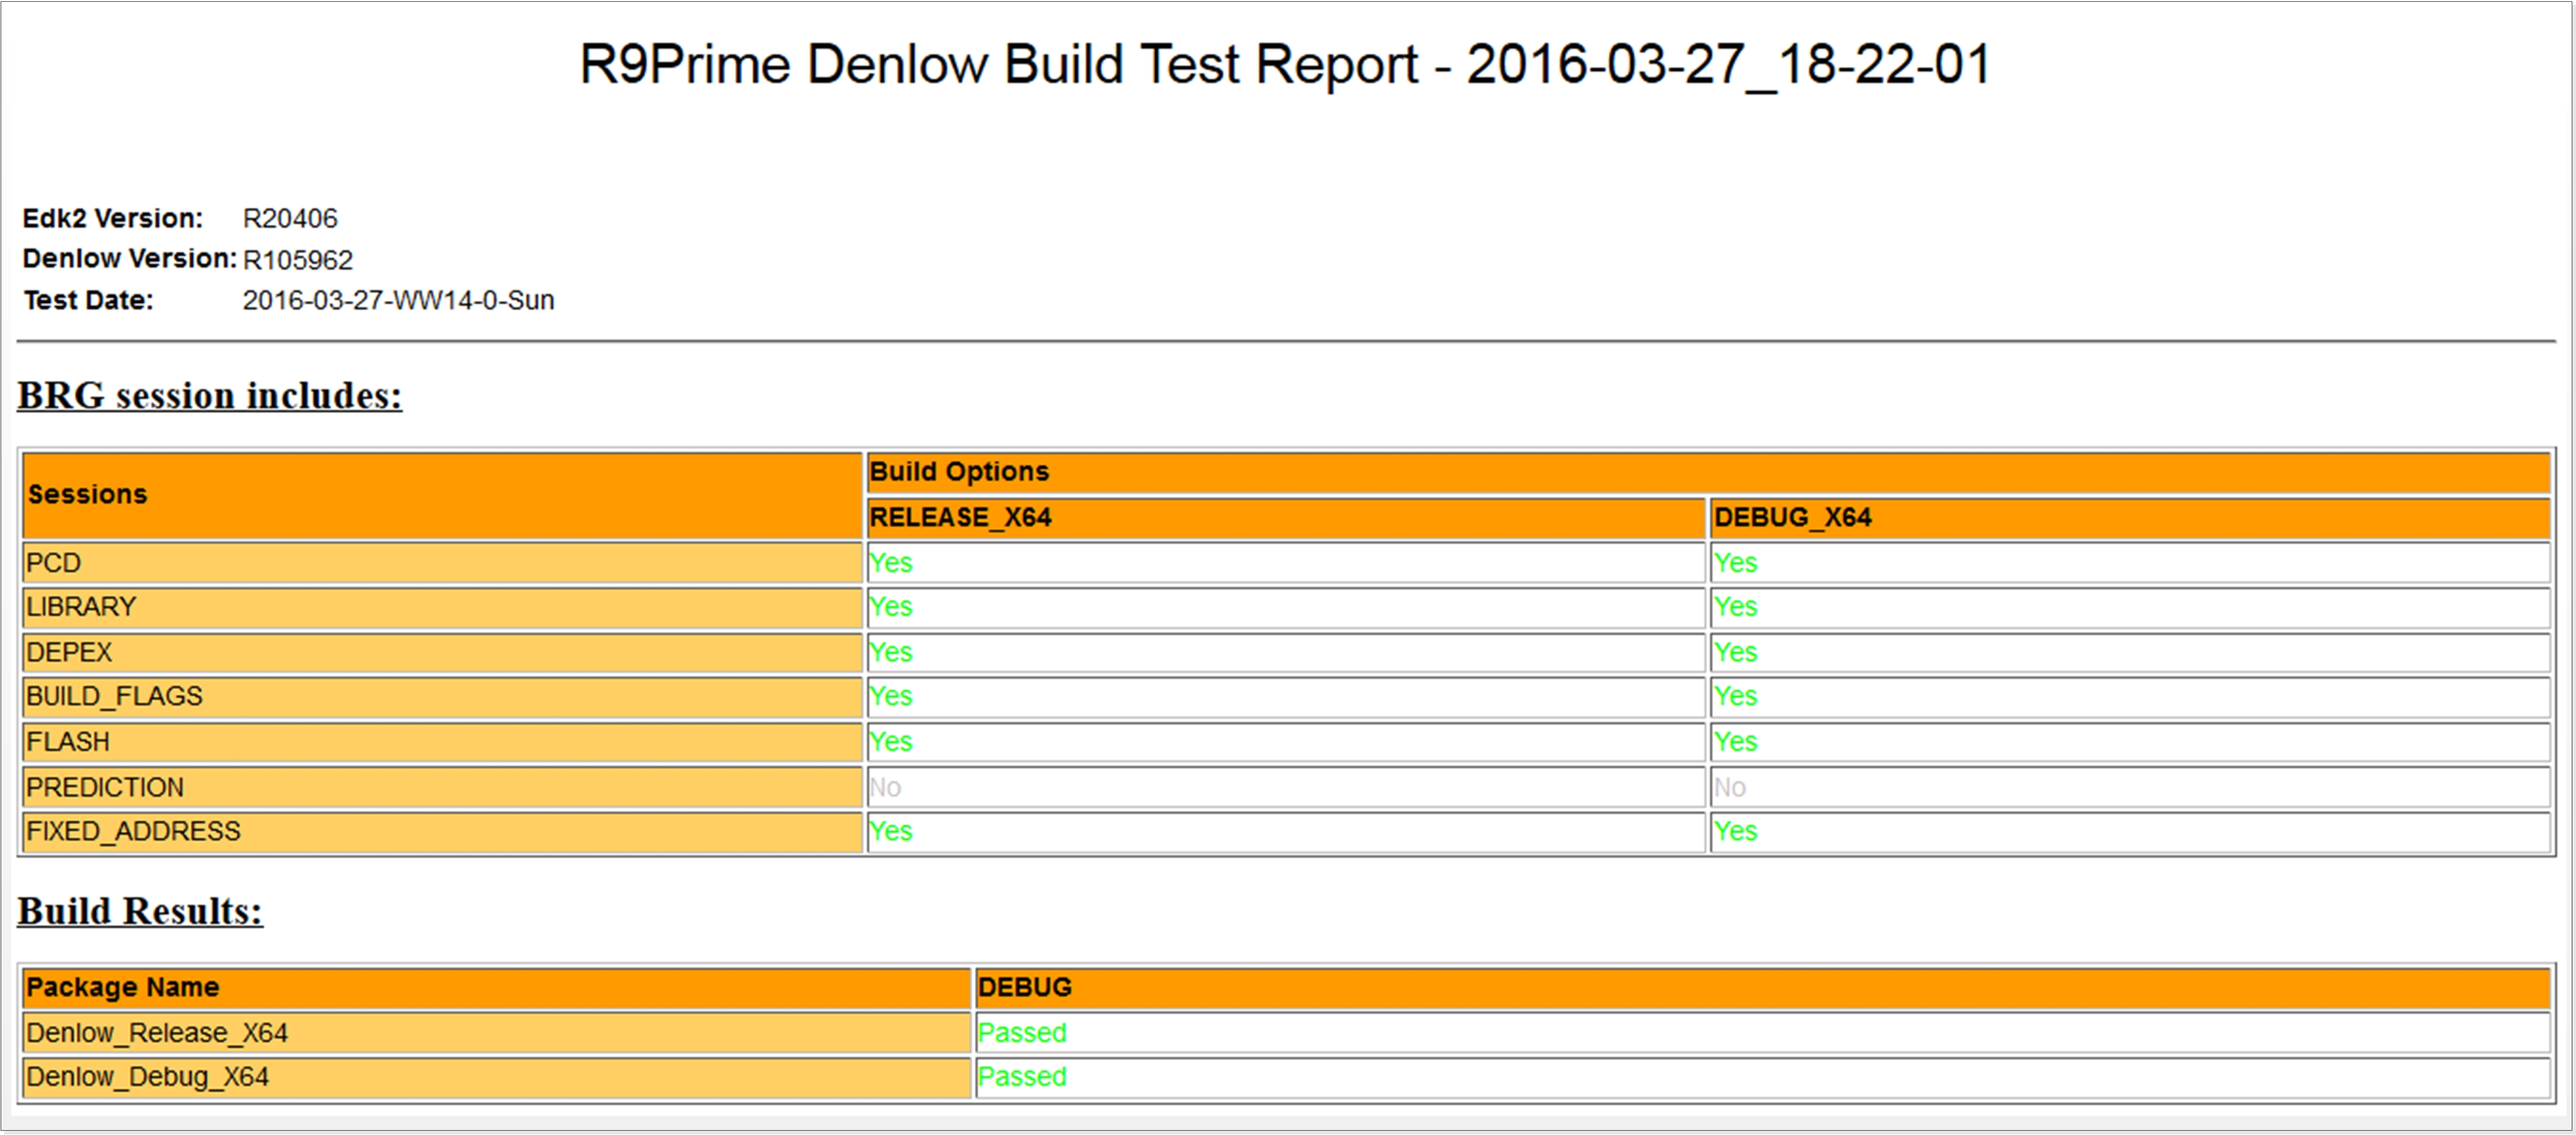
\includegraphics[height=7cm]{chart4/R9Prime-Denlow-Build-X64-Report-Edk2-R20406-R9-R105962}
					\caption{R9Prime-Denlow-Build-X64-Report-Edk2-R20406-R9-R105962}
					\label{fig:R9Prime-Denlow-Build-X64-Report-Edk2-R20406-R9-R105962}
				\end{figure}
					
			\item 产品测试报告
				
				产品测试报告主要负责对SCT执行的结果进行分析与总结。以R20311版本的Edk2与R105253版本的Denlow为例,其产品测试报告的结果如图~\ref{fig:R9Prime-Protocol-Test-for-Denlow-Edk2-R20311-R9-R105253}所示:
				
				\begin{figure}[H] % use float package if you want it here
					\centering
					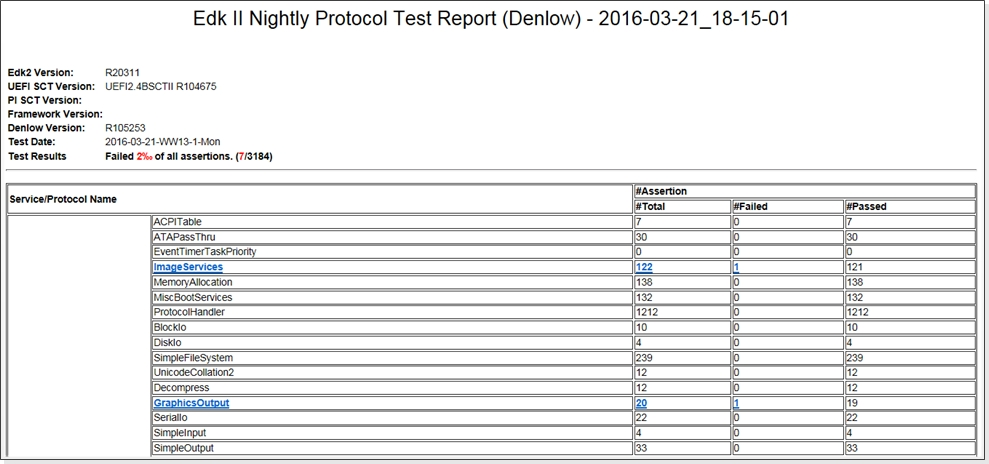
\includegraphics[height=7cm]{chart4/R9Prime-Protocol-Test-for-Denlow-Edk2-R20311-R9-R105253}
					\caption{R9Prime-Protocol-Test-for-Denlow-Edk2-R20311-R9-R105253}
					\label{fig:R9Prime-Protocol-Test-for-Denlow-Edk2-R20311-R9-R105253}
				\end{figure}
				
		\end{itemize}
	\subsection{实验结果分析与小结}
		\begin{itemize}
			\item 系统运行时间
				
				系统运行时间主要用于衡量系统运行的效率,短时间和高效率的系统运行是保障系统能够做到持续的基础。以R20406版本的Edk2、R105962版本的Denlow为例,依据其测试日志文件中的相关信息,该版本下持续集成测试系统的运行时间如表~\ref{tab:Edk2-R20406-Denlow-R105962版本的持续集成测试的运行时间}所示:
				
				\begin{longtable}[c]{c*{3}{r}}
					\caption{Edk2-R20406-Denlow-R105962版本的持续集成测试的运行时间}
					\label{tab:Edk2-R20406-Denlow-R105962版本的持续集成测试的运行时间}\\
					\toprule[1.5pt]
					 测试类型 & \multicolumn{1}{c}{起始时间} & \multicolumn{1}{c}{结束时间} & \multicolumn{1}{c}{耗时} \\\midrule[1pt]
					\endfirsthead
					\multicolumn{4}{c}{续表~\thetable\hskip1em 实验数据}\\
					\toprule[1.5pt]
					 测试类型 & \multicolumn{1}{c}{起始时间} & \multicolumn{1}{c}{结束时间} & \multicolumn{1}{c}{耗时} \\\midrule[1pt]
					\endhead
					\hline
					\multicolumn{4}{r}{续下页}
					\endfoot
					\endlastfoot
					Denlow-Build-X64 & 18:22:01.25 & 19:51:50.86 & 01:29:49.61 \\
					Protocol-Test-for-Denlow & 19:51:50.90 & 00:15:30.19 & 04:23:39.29 \\
					总计 & 18:22:01.25 & 00:15:30.19 & 05:53:28.90 \\
					\bottomrule[1.5pt]
				\end{longtable}
				
				从表中可以看出,Denlow-X64持续集成测试系统的运行耗时大概在六小时左右。由于其较为费时,因此采用每日集成策略,在无人值守的夜晚,自动化运行该系统,以对当前版本的产品进行测试,这样能够大大提高测试的效率,保障项目的高效进行。
			\item 系统运行成功率
				
				系统运行成功率主要用于衡量系统的稳定性和可靠性,高成功率是保障系统稳定性和可靠性的基础,也只有高成功率的系统才能更高程度的节省测试人员的测试时间,提高他们的测试效率。以该系统应用到项目开发后,其在一月份、二月份的执行统计为基础,其成功率如表~\ref{tab:Denlow-X64持续集成测试系统的运行成功率}所示:
				
				\begin{longtable}[c]{c*{3}{r}}
					\caption{Denlow-X64持续集成测试系统的运行成功率}
					\label{tab:Denlow-X64持续集成测试系统的运行成功率}\\
					\toprule[1.5pt]
					 月份 & \multicolumn{1}{c}{成功次数} & \multicolumn{1}{c}{失败次数} & \multicolumn{1}{c}{成功率} \\\midrule[1pt]
					\endfirsthead
					\multicolumn{4}{c}{续表~\thetable\hskip1em 实验数据}\\
					\toprule[1.5pt]
					 月份 & \multicolumn{1}{c}{成功次数} & \multicolumn{1}{c}{失败次数} & \multicolumn{1}{c}{成功率} \\\midrule[1pt]
					\endhead
					\hline
					\multicolumn{4}{r}{续下页}
					\endfoot
					\endlastfoot
					1月 & 28 & 3 & 90.3\% \\
					2月 & 27 & 2 & 93.1\% \\
					总计 & 55 & 5 & 91.7\% \\
					\bottomrule[1.5pt]
				\end{longtable}
				
				从表中可以看出,Denlow-X64持续集成测试系统的运行成功率能够保证在九成以上,这样绝大多数情况下系统均能够正常运行,测试人员只需要在第二天白天对系统测试的结果进行分析和报告即可,能够大大提高测试人员的效率;但是不可避免的仍然有少数情况系统未能够正常运行,其失败原因如表~\ref{tab:一、二月份Denlow-X64持续集成测试系统运行失败原因分析}所示:
				
				\begin{longtable}[c]{c*{3}{r}}
					\caption{一、二月份Denlow-X64持续集成测试系统运行失败原因分析}
					\label{tab:一、二月份Denlow-X64持续集成测试系统运行失败原因分析}\\
					\toprule[1.5pt]
					 系统运行失败原因 & \multicolumn{1}{c}{失败次数} & \multicolumn{1}{c}{失败原因类型} \\\midrule[1pt]
					\endfirsthead
					\multicolumn{4}{c}{续表~\thetable\hskip1em 实验数据}\\
					\toprule[1.5pt]
					 系统运行失败原因 & \multicolumn{1}{c}{失败次数} & \multicolumn{1}{c}{失败原因类型} \\\midrule[1pt]
					\endhead
					\hline
					\multicolumn{4}{r}{续下页}
					\endfoot
					\endlastfoot
					网络问题 & 2 & 系统外部因素  \\
					SVN服务器宕机 & 1 & 系统外部因素  \\
					产品源代码问题 & 2 & 产品质量因素  \\
					\bottomrule[1.5pt]
				\end{longtable}
				
				通过表中对失败原因进行的分析可以看出,系统失败的因素全部为系统外部因素所致。除了网络问题、源代码服务器问题以外,存在着开发过程中对源文件的修改不正确导致产品构建失败的因素,这也正是CI系统能够在第一时间的发现产品集成的问题这一重要意义的体现。
		\end{itemize}

\section{本章小结}
    这一章主要讲述了Denlow-X64持续集成测试系统的设计与实现,并且对实验结果进行了分析和总结。目前该套系统已经成功通过验证,并且部署应用到Denlow-X64的开发项目中,用于在其敏捷开发的过程中完成每日集成和测试产品的任务,从而尽早、及时的发现Denlow-X64中可能存在的缺陷,提高整个项目的开发效率。
	
